\begin{name}
	{Biên soạn: Thầy Lê Hồng Phi và Ninh Tiến Nam \& Phản biện: Thầy Ninh Tiến Nam và Lê Hồng Phi}
	{Đề thi giữa học kỳ I trường THPT Nguyễn Dục - Quảng Nam, năm 2020 - 2021}
\end{name}
	\setcounter{ex}{0}\setcounter{bt}{0}
	\Opensolutionfile{ans}[ans/ans-2-GHK1-29-NguyenDuc-QuangNam-21]
\begin{ex}%[Thi giữa học kỳ I, Trường THPT Nguyễn Dục - Quảng Nam, 2021]%[Lê Hồng Phi, 12EX3]%[2D1Y1-2]
Cho hàm số $y=f(x)$ có bảng biến thiên như sau
\begin{center}

\begin{tikzpicture}
\tkzTabInit[nocadre=false, lgt=1.2, espcl=2.5, deltacl=0.6]{$x$/0.6,$y'$/0.6,$y$/2}
{$-\infty$, $-4$, $0$, $4$, $+\infty$}
\tkzTabLine {,-,0,+,0,-,0,+,}
\tkzTabVar{+/$+\infty$,-/$-2$, +/$3$, -/$-2$, +/$+\infty$}
\end{tikzpicture}
\end{center}
Hàm số $y=f(x)$ đồng biến trên khoảng nào sau đây?
\choice
{$(0;+\infty)$}
{$(-2;+\infty)$}
{$(-2;3)$}
{\True $(-4;0)$}
\loigiai
{Theo bảng biến thiên, hàm số $y=f(x)$ đồng biến trên khoảng $(-4;0)$.
}
\end{ex}

\begin{ex}%[Thi giữa kỳ 1, trường THPT Nguyễn Dục,Sở GD và ĐT - Quảng Nam, năm 2020 - 2021]%[Ninh Tiến Nam, 12EX32021]%[2D1Y2-1]
	Cho hàm số $y=f(x)$ có $y'=(x-3)^3(2x+1)^2(3x+1)$. Tìm số điểm cực trị của hàm số $y=f(x)$.
	\choice
	{$4$}{$6$}{\True $2$}{$3$}
	\loigiai{
	Ta có
	\[y'=(x-3)^3(2x+1)^2(3x+1)=0\Leftrightarrow \heva{&x=3\\&x=-\dfrac{1}{2}\\&x=-\dfrac{1}{3}.}\]
	Bảng biến thiên của hàm số $f$ có dạng như sau
	\begin{center}
		\begin{tikzpicture}[line join=round, line cap=round,>=stealth,xscale=1.2,yscale=.8]
		\begin{scope}[shift={(-.5,.5)}]
		\def\a{10}
		\def\b{5}
		\draw (0,0) rectangle+(\a,-\b)
		(0,-1)--+(0:\a)
		(0,-2)--+(0:\a)
		(1,0)--+(-90:\b)
		
		;
		\end{scope}
		\path (0,0)node{$x$}+(1,0)node{$-\infty$}+(2.9,0)node[scale=.8]{$-\dfrac{1}{2}$}  +(4.9,0)node[scale=.8]{$-\dfrac{1}{3}$}+(7,0)node[scale=.9]{$3$}+(9,0)node{$+\infty$}
		++(0,-1)node{$f'$}
		+(2,0)node{$+$}
		+(3,0)node{$0$}
		+(4,0)node{$+$}
			+(5,0)node{$0$}
		+(6,0)node{$-$}+(7,0)node{$0$}
			+(8,0)node{$+$}
		++(0,-1.5)node{$f$}
		(1,-4)node (A){$-\infty$}
	
		
		(5,-2.1)node (C){}
		(7,-3.7)node (D){}
		(9,-2.1)node (E){$+\infty$}
		;
		\draw[->] (A)--(C);
	
		\draw[->] (C)--(D);
	\draw[->] (D)--(E);
		\end{tikzpicture}
		
	\end{center}
Vậy hàm số có $2$ điểm cực trị là $-\dfrac{1}{3}$ và $3$.			}
\end{ex}

\begin{ex}%[Thi giữa học kỳ I, Trường THPT Nguyễn Dục - Quảng Nam, 2021]%[Lê Hồng Phi, 12EX3]%[2D1Y2-2]
Cho hàm số $f(x)$ có bảng biến thiên như sau
\begin{center}

\begin{tikzpicture}
\tkzTabInit[nocadre=false, lgt=1.2, espcl=2.5, deltacl=0.6]{$x$/0.6,$f'(x)$/0.6,$f(x)$/2}
{$-\infty$, $-1$, $2$, $+\infty$}
\tkzTabLine {,-,0,+,0,-,}
\tkzTabVar{+/$+\infty$, -/$-3$, +/$1$, -/$-\infty$}
\end{tikzpicture}
\end{center}
Hàm số đã cho đạt cực tiểu tại điểm nào sau đây?
\choice
{$x=1$}
{\True $x=-1$}
{$x=-3$}
{$x=2$}
\loigiai
{Dựa vào bảng biến thiên, hàm số đã cho đạt cực tiểu tại điểm $x=-1$.
}
\end{ex}

\begin{ex}%[Thi giữa học kỳ I, Trường THPT Nguyễn Dục - Quảng Nam, 2021]%[Lê Hồng Phi, 12EX3]%[2D1Y4-1]
Đồ thị hàm số $y=\dfrac{3+2x}{2x-2}$ có các đường tiệm cận đứng và tiệm cận ngang. Hãy chọn phát biểu đúng.
\choice
{Tiệm cận đứng $x=-2$}
{Tiệm cận ngang $y=\dfrac{3}{2}$}
{Tiệm cận đứng $x=2$}
{\True Tiệm cận ngang $y=1$}
\loigiai
{Tập xác định $\mathscr{D}=\mathbb{R}\setminus \{1\}$.\\
Ta có
\begin{itemize}
\item $\lim\limits_{x\to 1^-}y=-\infty$, $\lim\limits_{x\to 1^+}y=+\infty$ nên đồ thị hàm số có tiệm cận đứng là $x=1$.
\item $\lim\limits_{x\to -\infty} y=\lim\limits_{x\to +\infty} y=1$ nên đồ thị hàm số có tiệm cận ngang là $y=1$.
\end{itemize}
}
\end{ex}

\begin{ex}%[Thi giữa học kỳ I, Trường THPT Nguyễn Dục - Quảng Nam, 2021]%[Lê Hồng Phi, 12EX3]%[2D1Y4-1]
Cho hàm số $y=f(x)$ có bảng biến thiên như hình bên dưới. 
\begin{center}

\begin{tikzpicture}
\tkzTabInit[nocadre=false, lgt=1.2, espcl=2.5, deltacl=0.6]{$x$/0.6,$y'$/0.6,$y$/2}
{$-\infty$, $-2$, $1$, $+\infty$}
\tkzTabLine {,-,d,-,d,+,}
\tkzTabVar{+/$4$, -D+/$1$/$+\infty$, -D-/$2$/$2$, +/$+\infty$}
\end{tikzpicture}
\end{center}
Đồ thị hàm số $y=f(x)$ có tất cả bao nhiêu đường tiệm cận (đứng và ngang)?
\choice
{\True $2$}
{$0$}
{$3$}
{$1$}
\loigiai
{Tập xác định $\mathscr{D}=\mathbb{R}\setminus\{-2;1\}$.\\Từ bảng biến thiên ta có 
\begin{itemize}
\item $\lim\limits_{x\to +\infty} y=+\infty$, $\lim\limits_{x\to -\infty} y=4$ nên đồ thị hàm số có một đường tiệm cận ngang $y=4$,
\item $\lim\limits_{x\to 1^-}y=2$, $\lim\limits_{x\to 1^+}y=2$, $\lim\limits_{x\to -2^+}y=+\infty$ nên đồ thị hàm số có một đường tiệm cận đứng $x=-2$.
\end{itemize}
Vậy đồ thị hàm số $y=f(x)$ có tất cả hai đường tiệm cận (đứng và ngang).
}
\end{ex}

\begin{ex}%[Thi giữa học kỳ I, Trường THPT Nguyễn Dục - Quảng Nam, 2021]%[Lê Hồng Phi, 12EX3]%[2D1Y5-3]
\immini{Cho hàm số $y=f(x)$ có đồ thị như hình bên. Tìm số nghiệm của phương trình $f(x)=-2$.
\choice
{$1$}
{$4$}
{\True $3$}
{$2$}}{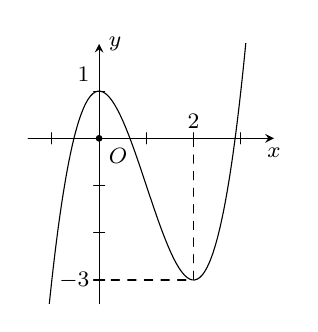
\begin{tikzpicture}[scale=1, font=\footnotesize, line join=round, line cap=round,>=stealth,x=0.6cm,y=0.6cm]
\def \xmin{-1.5};
\def \xmax{3.7};
\def \ymin{-3.5};
\def \ymax{2.0};
\draw[->] (\xmin, 0.) -- (\xmax,0.) node[anchor=north] {$x$};
\draw[->] (0.,\ymin) -- (0.,\ymax) node[anchor=west] {$y$};
\clip(\xmin,\ymin) rectangle (\xmax,\ymax);
\draw[smooth,samples=100,domain=\xmin-0.1:\xmax-0.1] plot(\x,{(\x)^3-3*(\x)^2+1});
\draw[dashed] (2,0) node[above] {$2$} -- (2,-3)--(0,-3)node[left] {$-3$} (0,1)node[above left]{$1$};
\foreach \x in {-4,-3,-2,-1,1,2,3,4}\draw (\x , 2pt)--(\x , -2pt);
\foreach \y in {-3,-2,-1,1}\draw (2pt, \y) -- (-2pt, \y);
\draw[fill=black] (0,0) circle (1pt) node[below right] {$O$};
\end{tikzpicture}}
\loigiai
{\immini{Số nghiệm của phương trình $f(x)=-2$ bằng số giao điểm giữa đồ thị hàm số $y=f(x)$ và đường thẳng $y=-2$.\\
Dựa vào đồ thị, đường thẳng $y=-2$ cắt đồ thị hàm số $y=f(x)$ tại $3$ điểm phân biệt.\\
Vậy phương trình $f(x)=-2$ có $3$ nghiệm phân biệt.}{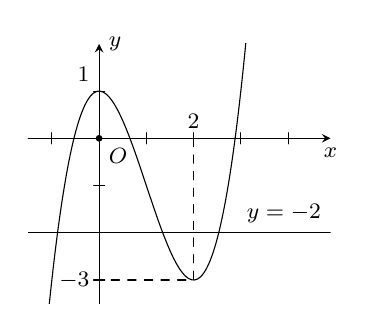
\begin{tikzpicture}[scale=1, font=\footnotesize, line join=round, line cap=round,>=stealth,x=0.6cm,y=0.6cm]
\def \xmin{-1.5};
\def \xmax{4.9};
\def \ymin{-3.5};
\def \ymax{2.0};
\draw[->] (\xmin, 0.) -- (\xmax,0.) node[anchor=north] {$x$};
\draw[->] (0.,\ymin) -- (0.,\ymax) node[anchor=west] {$y$};
\clip(\xmin,\ymin) rectangle (\xmax,\ymax);
\draw[smooth,samples=100,domain=\xmin-0.1:\xmax-0.1] plot(\x,{(\x)^3-3*(\x)^2+1});
\draw[dashed] (2,0) node[above] {$2$} -- (2,-3)--(0,-3)node[left] {$-3$} (0,1)node[above left]{$1$} ;
\draw (\xmin,-2)--(\xmax,-2)  node[above left]{$y=-2$}; 
\foreach \x in {-4,-3,-2,-1,1,2,3,4}\draw (\x , 2pt)--(\x , -2pt);
\foreach \y in {-3,-2,-1,1}\draw (2pt, \y) -- (-2pt, \y);
\draw[fill=black] (0,0) circle (1pt) node[below right] {$O$};
\end{tikzpicture}}
}
\end{ex}

\begin{ex}%[Thi giữa học kỳ I, Trường THPT Nguyễn Dục - Quảng Nam, 2021]%[Lê Hồng Phi, 12EX3]%[2H1Y1-2]
Số đỉnh của một khối lăng trụ tam giác là 
\choice
{\True $6$}
{$8$}
{$12$}
{$4$}
\loigiai
{\immini{Số đỉnh của một khối lăng trụ tam giác là $6$.}{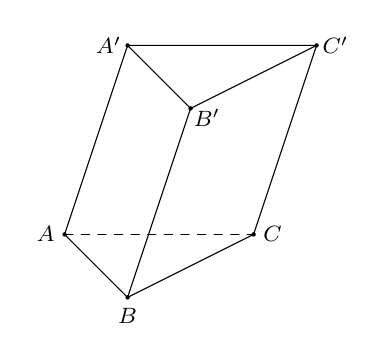
\begin{tikzpicture}[scale=0.8, font=\footnotesize, line join=round, line cap=round,>=stealth]
\path (0,0)coordinate (A) (3,0) coordinate (C) (1,-1) coordinate (B) (1,3) coordinate (h);
\foreach \p in {A,B,C} {\draw (\p)--(\p)--+(h) coordinate (\p');}
\draw (A')--(B')--(C')--cycle (A)--(B)--(C);
\draw[dashed] (A)--(C);
\foreach \p/\g in {A/180,B/-90,C/0,A'/180,B'/-30,C'/0} \fill[black] (\p) circle(1pt)+(\g:0.3) node{$\p$};
\end{tikzpicture}}
}
\end{ex}

\begin{ex}%[Thi giữa học kỳ I, Trường THPT Nguyễn Dục - Quảng Nam, 2021]%[Lê Hồng Phi, 12EX3]%[2H1Y2-2]
Khối lập phương là khối đa diện đều thuộc loại nào sau đây?
\choice
{$\{3;3\}$}
{\True $\{4;3\}$}
{$\{3;5\}$}
{$\{3;4\}$}
\loigiai
{\immini{Mỗi mặt của khối lập phương là tứ giác đều, mỗi đỉnh của khối lập phương là đỉnh chung của đúng $3$ mặt.\\
Vậy khối lập phương là khối đa diện đều loại $\{4;3\}$.}{\begin{tikzpicture}[scale=1, font=\footnotesize, line join=round, line cap=round,>=stealth]
\path (0,2) coordinate (h) (0,0)coordinate (B) (2,0) coordinate (C) (3,1) coordinate (D) ($(B)+(D)-(C)$) coordinate (A);
\foreach \p in {A,B,C,D}\path ($(\p)+(h)$) coordinate (\p');
\draw (A')--(B')--(B)--(C)--(D)--(D')--cycle (B')--(C')--(D') (C)--(C');
\draw[dashed] (B)--(A)--(D) (A)--(A');
\foreach \p/\g in {A/150,B/240,C/-60,D/0,A'/90,B'/180,C'/-30,D'/45} \fill[black] (\p) circle(1pt)+(\g:0.3) node{$\p$};
\end{tikzpicture}}
}
\end{ex}

\begin{ex}%[Thi giữa kỳ 1, trường THPT Nguyễn Dục,Sở GD và ĐT - Quảng Nam, năm 2020 - 2021]%[Ninh Tiến Nam, 12EX32021]%[2H1Y2-2]
Tổng số đỉnh, số cạnh, số mặt của bát diện đều là	
	\choice
	{$30$}{$28$}{$14$}{\True $26$}
	\loigiai{
	\immini{	Bát diện đều có tổng số đỉnh, số cạnh, số mặt bằng $6+12+8=26$.}{
		\begin{tikzpicture}[>=stealth,line join=round,line cap=round,font=\footnotesize,scale=1]
	\tkzDefPoints{0/0/O, -.5/.4/A, 1.5/.4/B}
	\coordinate (S) at ($(O)+(0,1.5)$);
	\tkzDefPointBy[symmetry = center O](A) \tkzGetPoint{C}
	\tkzDefPointBy[symmetry = center O](B) \tkzGetPoint{D}
	\tkzDefPointBy[symmetry = center O](S) \tkzGetPoint{S'}
	\tkzDrawSegments[dashed](S,A A,B A,D A,S')
	\tkzDrawPolygon(S,C,D)
	\tkzDrawPolygon(S',B,C)
	\tkzDrawSegments(S,B S',D)
		\end{tikzpicture}}
	}
\end{ex}

\begin{ex}%[Thi giữa học kỳ I, Trường THPT Nguyễn Dục - Quảng Nam, 2021]%[Lê Hồng Phi, 12EX3]%[2H1Y3-2]
Thể tích khối chóp có diện tích đáy  $B$ và chiều cao $h$ bằng
\choice
{$Bh$}
{$\dfrac{1}{2}Bh$}
{\True $\dfrac{1}{3}Bh$}
{$3Bh$}
\loigiai
{Thể tích khối chóp có diện tích đáy  $B$ và chiều cao $h$ là $V=\dfrac{1}{3}Bh$.
}
\end{ex}

\begin{ex}%[Thi giữa học kỳ I, Trường THPT Nguyễn Dục - Quảng Nam, 2021]%[Lê Hồng Phi, 12EX3]%[2H1Y3-2]
Cho khối lăng trụ có thể tích $V$, diện tích đáy $S$. Chiều cao lăng trụ $h$ bằng
\choice
{\True $h=\dfrac{V}{S}$}
{$h=\dfrac{S}{V}$}
{$h=\dfrac{3V}{S}$}
{$h=V\cdot S$}
\loigiai
{Thể tích của khối lăng trụ là $V=Sh$ nên chiều cao của khối lăng trụ là $h=\dfrac{V}{S}$.
}
\end{ex}

\begin{ex}%[Thi giữa học kỳ I, Trường THPT Nguyễn Dục - Quảng Nam, 2021]%[Lê Hồng Phi, 12EX3]%[2H1Y3-2]
Thể tích khối lập phương cạnh $2a$ là 
\choice
{\True $8a^3$}
{$a^3$}
{$\dfrac{1}{8}a^3$}
{$6a^3$}
\loigiai
{Thể tích khối lập phương cạnh $2a$ là $V=(2a)^3=8a^3$.
}
\end{ex}

\begin{ex}%[Thi giữa kỳ 1, trường THPT Nguyễn Dục,Sở GD và ĐT - Quảng Nam, năm 2020 - 2021]%[Ninh Tiến Nam, 12EX32021]%[2H1Y3-2]
	Cho khối chóp $S.ABCD$ có đáy là hình vuông cạnh $2a$, $SA\perp (ABCD)$ và $SA=a$. Thể tích khối chóp $S.ABCD$ bằng
	\choice
	{$\dfrac{a^3}{3}$}{\True $\dfrac{4a^3}{3}$}{$\dfrac{2a^3}{3}$}{$4a^3$}
	\loigiai{
\immini{		Thể tích khối chóp $S.ABCD$ bằng
		\[V=\dfrac{1}{3}\cdot SA\cdot S_{ABCD}=\dfrac{1}{3}\cdot a\cdot (2a)^2=\dfrac{4a^3}{3}.\]}{\begin{tikzpicture}[>=stealth,line join=round,line cap=round,font=\footnotesize,scale=.9]
		\path 
		(0,0)coordinate (A)
		+(-45:1.82)coordinate (B)
		+	(180:2.5)coordinate (D)
		($(D)+(B)-(A)$)coordinate (C)
		(A)+(90:2)coordinate (S)
		
		;
		\draw [dashed] (S)--(A)--(B) (D)--(A)  ;
		\draw (S)--(D)--(C)--(B)--cycle (S)--(C);
		\foreach \x/\g in {S/90,A/20,B/0,C/-120,D/180}\fill (\x)circle (0.04)+(\g:3mm)node[scale=.9]{$\x$};
	
		\end{tikzpicture}}
			}
\end{ex}

\begin{ex}%[Thi giữa học kỳ I, Trường THPT Nguyễn Dục - Quảng Nam, 2021]%[Lê Hồng Phi, 12EX3]%[2D1B1-1]
Trong các hàm số sau, hàm số nào đồng biến trên khoảng $(-\infty;+\infty)$?
\choice
{\True $y=x^3+x^2+x+1$}
{$y=x^4+2x^2+1$}
{$y=-x^3+2x^2-x+1$}
{$y=3x^2+1$}
\loigiai
{Ta có \begin{itemize}
\item $y=x^4+2x^2+1$ là hàm số trùng phương nên không đồng biến trên $(-\infty;+\infty)$,
\item $y=3x^2+1$ là hàm số bậc hai nên không đồng biến trên $(-\infty;+\infty)$,
\item $y=-x^3+2x^2-x+1$ có $\lim\limits_{x\to +\infty}y=-\infty$ nên không đồng biến trên $(-\infty;+\infty)$,
\item $y=x^3+x^2+x+1$ có $y'=3x^2+2x+1=2x^2+(x+1)^2>0,\ \forall x\in (-\infty;+\infty)$ nên đồng biến trên $(-\infty;+\infty)$.
\end{itemize}
}
\end{ex}

\begin{ex}%[Thi giữa kỳ 1, trường THPT Nguyễn Dục,Sở GD và ĐT - Quảng Nam, năm 2020 - 2021]%[Ninh Tiến Nam, 12EX32021]%[2D1B1-3]
Điều kiện của tham số $m$ để hàm số $y=\dfrac{2mx+1}{x-2}$ đồng biến trên từng khoảng xác định của nó là
	\choice
	{\True $m<\dfrac{-1}{4}$}{$m\ge \dfrac{-1}{4}$}{$m>\dfrac{-1}{4}$}{$m\le \dfrac{-1}{4}$}
	\loigiai{
Hàm số 	$y=\dfrac{2mx+1}{x-2}$ xác định trên $\mathscr{D}=(-\infty;2)\cup (2;+\infty)$, $y'=-\dfrac{4m+1}{(x-2)^2}$, với mọi $x\in\mathscr{D}$.\\ Do đó, hàm số đã cho đồng biến trên từng khoảng xác định của nó khi và chỉ khi
\[y'>0,\ \forall x\in \mathscr{D}\Leftrightarrow 4m+1<0\Leftrightarrow m<\dfrac{-1}{4}.\]
}
\end{ex}

\begin{ex}%[Thi giữa học kỳ I, Trường THPT Nguyễn Dục - Quảng Nam, 2021]%[Lê Hồng Phi, 12EX3]%[2D1B2-1]
Đồ thị hàm số nào dưới đây có $3$ điểm cực trị?
\choice
{$y=-x^4-3x^2+2$}
{\True $y=x^4-3x^2+1$}
{$y=x^4+3x^2+1$}
{$y=x^3+3x+1$}
\loigiai
{Hàm số bậc ba có tối đa $2$ điểm cực trị.\\
Hàm số trùng phương $y=ax^4+bx^2+c$ ($a\neq 0$) có $3$ điểm cực trị khi và chỉ khi $ab<0$.\\
Vậy trong các phương án đã cho thì đồ thị hàm số $y=x^4-3x^2+1$ có $3$ điểm cực trị.
}
\end{ex}

\begin{ex}%[Thi giữa học kỳ I, Trường THPT Nguyễn Dục - Quảng Nam, 2021]%[Lê Hồng Phi, 12EX3]%[2D1B3-1]
Tìm giá trị lớn nhất của hàm số $y=\dfrac{-x+1}{-2x+3}$ trên đoạn $[-2;1]$.
\choice
{\True $\dfrac{3}{7}$}
{$-1$}
{$-\dfrac{1}{49}$}
{$0$}
\loigiai
{Hàm số đã cho xác định và liên tục trên đoạn $[-2;1]$.\\
Ta có $y'=-\dfrac{1}{(-2x+3)^2}<0,\ \forall x \in [-2;1]$. Suy ra hàm số nghịch biến trên $[-2;1]$.\\
Vậy $\max\limits_{[-2;1]} y=y(-2)=\dfrac{3}{7}$.
}
\end{ex}

\begin{ex}%[Thi giữa kỳ 1, trường THPT Nguyễn Dục,Sở GD và ĐT - Quảng Nam, năm 2020 - 2021]%[Ninh Tiến Nam, 12EX32021]%[2D1B3-1]
	Tìm giá trị lớn nhất của hàm số $y=x^3-3x$ trên $[-2;0]$.
	\choice
	{$0$}{$-2$}{$3$}{\True $2$}
	\loigiai{
Hàm số $y=x^3-3x$ xác định và liên tục trên  $[-2;0]$. Ta có	 $y'=3x^2-3$;
	\[y'=0\Leftrightarrow 3x^2-3=0\Leftrightarrow \heva{&x=-1\in [-2;0]\\&x=1\not\in [-2;0].}\]
Ta có $y(-2)=-2$, $y(-1)=2$, $y(0)=0$.\\
Vậy giá trị lớn nhất hàm số $y=x^3-3x$ trên $[-2;0]$ bằng $2$.
	}
\end{ex}

\begin{ex}%[Thi giữa kỳ 1, trường THPT Nguyễn Dục,Sở GD và ĐT - Quảng Nam, năm 2020 - 2021]%[Ninh Tiến Nam, 12EX32021]%[2D1B3-2]
Trên khoảng $(0;+\infty)$	 thì hàm số $y=-x^3+3x+1$
	\choice
{\True có giá trị lớn nhất bằng $3$}
{có giá trị nhỏ nhất bằng $3$}
{có giá trị nhỏ nhất bằng $-1$}
{có giá trị lớn nhất bằng $-1$}
	\loigiai{
\immini{Ta có $y'=-3x^2+3$,\[y'=0\Leftrightarrow-3x^2+3=0 \Leftrightarrow \heva{&x=1\in (0;+\infty)\\&x=-1\not\in (0;+\infty).}\]	
Bảng biến thiên của hàm số như hình bên.\\Vậy hàm số có giá trị lớn nhất trên khoảng $(0;+\infty)$ bằng $3$.}{	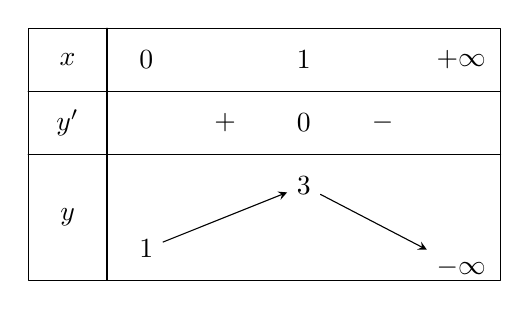
\begin{tikzpicture}[line join=round, line cap=round,>=stealth,xscale=1,yscale=.8]
\begin{scope}[shift={(-.5,.5)}]
\def\a{6}
\def\b{4}
\draw (0,0) rectangle+(\a,-\b)
(0,-1)--+(0:\a)
(0,-2)--+(0:\a)
(1,0)--+(-90:\b)

;
\end{scope}
\path (0,0)node{$x$}+(1,0)node{$0$}+(3,0)node{$1$}  +(5,0)node{$+\infty$}
++(0,-1)node{$y'$}
+(2,0)node{$+$}
+(3,0)node{$0$}
+(4,0)node{$-$}
%	+(5,0)node{$0$}
++(0,-1.5)node{$y$}
(1,-3)node (A){$1$}
(3,-2)node (B){$3$}
(5,-3.3)node (C){$-\infty$}

;
\draw[->] (A)--(B);
\draw[->] (B)--(C);
\end{tikzpicture}}
}
\end{ex}

\begin{ex}%[Thi giữa học kỳ I, Trường THPT Nguyễn Dục - Quảng Nam, 2021]%[Lê Hồng Phi, 12EX3]%[2D1B5-1]
\immini{Trong các hàm số sau đây, hàm số nào có đồ thị như hình vẽ bên? 
\choice
{$y=x^3-3x+1$}
{\True $y=-x^3+3x+1$}
{$y=x^3+2$}
{$y=-x^4+3x$}}{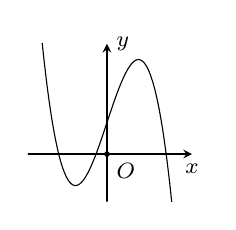
\begin{tikzpicture}[scale=0.8, font=\footnotesize, line join=round, line cap=round,>=stealth,x=0.5cm, y=0.5cm]
\def \xmin{-2.5};
\def \xmax{2.7};
\def \ymin{-1.5};
\def \ymax{3.5};
\draw[->] (\xmin, 0.) -- (\xmax,0.) node[anchor=north] {$x$};
\draw[->] (0.,\ymin) -- (0.,\ymax) node[anchor=west] {$y$};
\clip(\xmin,\ymin) rectangle (\xmax,\ymax);
\draw[smooth,samples=100,domain=\xmin-0.1:\xmax-0.1] plot(\x,{-(\x)^3+3*(\x)+1});
\draw[fill=black] (0,0) circle (1pt) node[below right] {$O$};
\end{tikzpicture}}
\loigiai
{Đồ thị trong hình vẽ không đi qua gốc tọa độ $O$ nên không phải là đồ thị của hàm số $y=-x^4+3x$. Do đó, dạng đồ thị trong hình vẽ là của hàm số $y=ax^3+bx^2+cx+d$ với $a\neq 0$.\\
Từ đồ thị ta thấy $\lim\limits_{x\to +\infty} y=-\infty$ nên $a<0$.\\
Vậy trong các phương án đã cho chỉ có hàm số $y=-x^3+3x+1$ có đồ thị phù hợp với hình vẽ.
}
\end{ex}

\begin{ex}%[Thi giữa học kỳ I, Trường THPT Nguyễn Dục - Quảng Nam, 2021]%[Lê Hồng Phi, 12EX3]%[2D1B5-4]
Đồ thị của hàm số $y=x^4-3x^2-4$ cắt trục hoành tại hai điểm  có hoành độ là $x_1$, $x_2$. Giá trị của biểu thức $x_1^2+x_2^2$ bằng
\choice
{$9$}
{$6$}
{\True $8$}
{$12$}
\loigiai
{Phương trình hoành độ giao điểm giữa đồ thị và trục hoành là $$
x^4-3x^2-4=0\Leftrightarrow\hoac{& x^2=-1 && (\text{vô nghiệm}) \\ & x^2=4}\Leftrightarrow \hoac{& x=-2 \\ & x=2.}$$
Vậy $x_1^2+x_2^2=8$.
}
\end{ex}

\begin{ex}%[Thi giữa kỳ 1, trường THPT Nguyễn Dục,Sở GD và ĐT - Quảng Nam, năm 2020 - 2021]%[Ninh Tiến Nam, 12EX32021]%[2H1B3-2]
	Thể tích khối lăng trụ tam giác đều có tất cả các cạnh bằng $2a$ bằng
	\choice
	{$2a^3$}{ $a^3\sqrt{3}$}{\True $2\sqrt{3}a^3$}{$\dfrac{2\sqrt{3}a^3}{3}$}	
	\loigiai{
		\immini{Xét khối lăng trụ tam giác đều $ABC.A'B'C$ có các cạnh bằng $2a$.\\Diện tích  đáy $ABC$ bằng 
			$S_{ABC}=\dfrac{(2a)^2\sqrt{3}}{4}=a^2\sqrt{3}$.\\
			Chiều cao của khối lăng trụ là $AA'=2a$.\\
			Vậy thể tích khối lăng trụ bằng \[V=S_{ABC}\cdot AA'=a^2\sqrt{3}\cdot 2a=2\sqrt{3}a^3.\]
		}{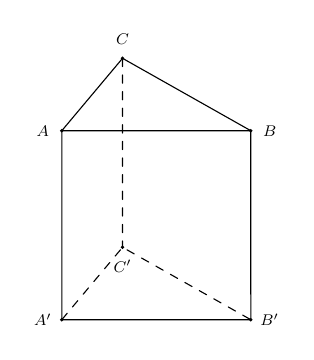
\begin{tikzpicture}[>=stealth,line join=round,line cap=round,font=\footnotesize,scale=.8]
		\path 
		(0,0)coordinate (A)
		+(0:3)coordinate (B)
		+(50:1.5)coordinate (C)
		(A)--+(-90:3)coordinate (A')
			(B)--+(-90:3)coordinate (B')
				(C)--+(-90:3)coordinate (C')
		;	
			\draw (A)--(B)--(C)--cycle (A')--(B') (A)--(A') (B)--(B');
			\draw[ dashed] (A')--(C')--(B') (C)--(C');
			\foreach \x/\g in {A/180,B/0,C/90,A'/180,B'/0,C'/-90}\fill (\x)circle (0.03)+(\g:3mm)node[scale=.7]{$\x$};
			\end{tikzpicture}}
		
		
	}
\end{ex}

\begin{ex}%[Thi giữa kỳ 1, trường THPT Nguyễn Dục,Sở GD và ĐT - Quảng Nam, năm 2020 - 2021]%[Ninh Tiến Nam, 12EX32021]%[1D5K2-2]
	Gọi $M(a;2a)$, $a>0$ là một điểm nằm trên đồ thị $(C)$ của hàm số $y=\dfrac{2x+6}{x-1}$. Tiếp tuyến của $(C)$ tại $M$ có hệ số góc là 
	\choice
	{$k=-8$}	{\True $k=-2$}	{$k=-1$}	{$k=-4$}
	\loigiai{
	Do $M(a;2a)\in (C)\colon y=\dfrac{2x+6}{x-1} $	nên
	\allowdisplaybreaks
	\begin{eqnarray*}
	2a=\dfrac{2a+6}{a-1}\Leftrightarrow \heva{&a\ne 1\\& 2a^2-4a-6=0}\Leftrightarrow \heva{&a\ne 1\\& a^2-2a-3=0}\Leftrightarrow \hoac{&a=-1\\&a=3.}
	\end{eqnarray*} 
	Theo giả thiết $a>0$ nên $a=3$, suy ra $M(3;6)$. Ta có $y'=-\dfrac{8}{(x-1)^2}$.\\
	Vậy  tiếp tuyến của $(C)$ tại $M$ có hệ số góc là $k=y'(3)=-2$.
	}
\end{ex}

\begin{ex}%[Thi giữa kỳ 1, trường THPT Nguyễn Dục,Sở GD và ĐT - Quảng Nam, năm 2020 - 2021]%[Ninh Tiến Nam, 12EX32021]%[2D1K1-3]
Cho hàm số $y=x^3-3x^2+mx+1$	với $m$ là tham số. Có bao nhiêu giá trị nguyên của $m$ thuộc khoảng $(0;5)$ để hàm số đồng biến trên $(0;+\infty)$?
	\choice
	{$1$}{$0$}{\True  $2$}{$4$}	
	\loigiai{
		Ta có $y'=3x^2-6x+m$. Hàm số đồng biến trên $(0;+\infty)$ khi và chỉ khi
		\[\heva{&y'\ge 0,\ \forall x>0\\&\text{phương trình}\ y'=0\ \text{có hữu hạn nghiệm}.}\]
	Điều kiện thứ hai là hiển nhiên đúng vì $y'=3x^2-6x+m=0$	 là phương trình bậc hai.\\
	Ta xét điều kiện thứ nhất
	\allowdisplaybreaks
	\begin{eqnarray*}
	&&y'=3x^2-6x+m\ge 0 ,\ \forall x>0\\
	&\Leftrightarrow& m-3\ge -3(x-1)^2 ,\ \forall x>0\\
	&\Leftrightarrow&m\ge 3.
	\end{eqnarray*}
Do $m$ nguyên và $m$ thuộc khoảng $(0;5)$ nên có $2$ giá trị của $m$ thỏa mãn là $m\in\{3;4\}$.	}
\end{ex}

\begin{ex}%[Thi giữa kỳ 1, trường THPT Nguyễn Dục,Sở GD và ĐT - Quảng Nam, năm 2020 - 2021]%[Ninh Tiến Nam, 12EX32021]%[2D1K2-2]
\immini{Cho hàm số $y=f(x)$ có đồ thị như hình vẽ. Tìm số điểm cực trị của hàm số $y=|f(x)|$.
	\choice
	{$4$}{$6$}{\True $2$}{$3$}	}{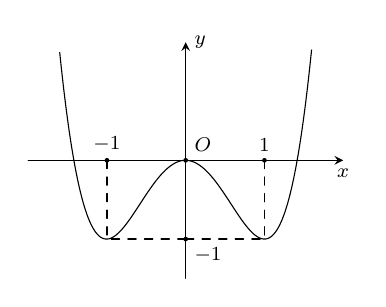
\begin{tikzpicture}[>=stealth,line join=round,line cap=round,font=\footnotesize,scale=1]
	\draw[->](-2,0)--(2,0)node[scale=.9,below]{$x$};
	\draw[->](0,-1.5)--(0,1.5)node[scale=.9,right]{$y$};
	\draw[domain=-1.6:1.6,samples=300] plot (\x,{0.99*(\x)^4+0.01*(\x)^3-1.99*(\x)^2-0.01*\x});
	\fill (0,0)  circle (0.03) node[scale=0.9, above right]{$O$}
	(-1,0)circle (0.03) node[scale=0.9, above]{$-1$}
	(1,0)circle (0.03) node[scale=0.9, above]{$1$}
	(0,-1)circle (0.03) node[scale=0.9, below right]{$-1$}
	;
	\draw[dashed] (-1,0)|-(0,-1)  (1,0)|-(0,-1) ;
	\end{tikzpicture}}
	\loigiai{
\immini{		Ta có 
		\[|f(x)|=\heva{&f(x),\ \text{nếu}\ f(x)\ge 0,\\
		&-f(x),\ \text{nếu}\ f(x)< 0.}\]
	Đồ thị hàm số $y=|f(x)|$ có dạng như hình vẽ bên.}{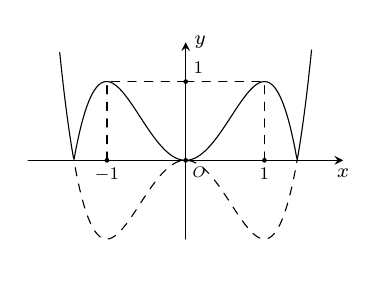
\begin{tikzpicture}[>=stealth,line join=round,line cap=round,font=\footnotesize,scale=1]
		\draw[->](-2,0)--(2,0)node[scale=.9,below]{$x$};
		\draw[->](0,-1)--(0,1.5)node[scale=.9,right]{$y$};
	\begin{scope}
	\draw[domain=-1.6:1.6,samples=300] plot (\x,{abs(0.99*(\x)^4+0.01*(\x)^3-1.99*(\x)^2-0.01*\x)});
	\end{scope}	
	\begin{scope}
	\clip (-2,0)rectangle (2,-1.5);
	\draw[domain=-1.6:1.6,samples=300,dashed] plot (\x,{0.99*(\x)^4+0.01*(\x)^3-1.99*(\x)^2-0.01*\x});
	\end{scope}	
		\fill (0,0)  circle (0.03) node[scale=0.7, below right]{$O$}
		(-1,0)circle (0.03) node[scale=0.8, below]{$-1$}
		(1,0)circle (0.03) node[scale=0.8, below]{$1$}
		(0,1)circle (0.03) node[scale=0.8, above right]{$1$}
		;
		\draw[dashed] (-1,0)|-(0,1)  (1,0)|-(0,1) ;
		\end{tikzpicture}}
\noindent Vậy hàm số  $y=|f(x)|$ có $5$ điểm cực trị.	}
\end{ex}

\begin{ex}%[Thi giữa kỳ 1, trường THPT Nguyễn Dục,Sở GD và ĐT - Quảng Nam, năm 2020 - 2021]%[Ninh Tiến Nam, 12EX32021]%[2D1K3-1]
Tìm $m$ để tổng giá trị lớn nhất và giá trị nhỏ nhất của hàm số	$y=\dfrac{2mx+1}{x+3}$ trên đoạn $[0;1]$ bằng $\dfrac{1}{3}$.
	\choice
	{\True $-\dfrac{1}{2}$}{$-\dfrac{1}{3}$}{\True $\dfrac{1}{3}$}{$\dfrac{1}{2}$}	
	\loigiai{
Trên $[0;1]$, ta có $y'=\dfrac{6m-1}{(x-3)^2}$.	
Vì  $y'$ không đổi dấu trên $[0;1]$ nên hàm số đạt giá trị lớn nhất và giá trị nhỏ nhất tại hai đầu mút của 	đoạn $[0;1]$.\\
Ta có \[y(0)+y(1)=\dfrac{1}{3}\Leftrightarrow \dfrac{1}{3}+\dfrac{2m+1}{4}=\dfrac{1}{3}\Leftrightarrow m=-\dfrac{1}{2}.\]	
Vậy $-\dfrac{1}{2}$ là giá trị cần tìm của $m$.	}
\end{ex}

\begin{ex}%[Thi giữa học kỳ I, Trường THPT Nguyễn Dục - Quảng Nam, 2021]%[Lê Hồng Phi, 12EX3]%[2D1K5-1]
\immini{Cho hàm số $y=f(x)=ax^3+bx^2+cx+d$, ($a, b, c, d\in\mathbb{R}$) có đồ thị như hình vẽ bên. Chọn khẳng định đúng trong các khẳng định sau.
\choice
{$a>0$, $b<0$, $d<0$}
{$a<0$, $b<0$, $d<0$}
{$a>0$, $b>0$, $d>0$}
{\True $a>0$, $b>0$, $d<0$}}{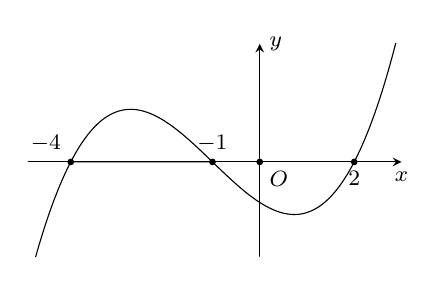
\begin{tikzpicture}[scale=1, font=\footnotesize, line join=round, line cap=round,>=stealth,x=0.6cm, y=0.6cm]
\def \xmin{-4.9};
\def \xmax{3.0};
\def \ymin{-2.0};
\def \ymax{2.5};
\draw[->] (\xmin, 0.) -- (\xmax,0.) node[anchor=north] {$x$};
\draw[->] (0.,\ymin) -- (0.,\ymax) node[anchor=west] {$y$};
\clip(\xmin,\ymin) rectangle (\xmax,\ymax);
\draw[smooth,samples=100,domain=\xmin-0.1:\xmax-0.1] plot(\x,{(3/28)*(\x)^3+(9/28)*(\x)^2-(9/14)*(\x)-6/7});
\draw[fill=black] (0,0) circle (1pt) node[below right] {$O$} (-4,0) circle (1pt) node[above left] {$-4$} -- (-1,0) circle (1pt) node[above] {$-1$} (2,0) circle (1pt) node[below]{2};
\end{tikzpicture}}
\loigiai
{Đồ thị cắt trục hoành tại $3$ điểm có hoành độ $x_1=-4$, $x_2=-1$, $x_3=2$ nên $a\neq 0$ và $$f(x)=a(x+4)(x+1)(x-2)=ax^3+3ax^2-6ax-8a.$$
Do đó $b=3a$ và $d=-8a$.\\
Từ đồ thị ta có $\lim\limits_{x\to +\infty} y=+\infty$ nên $a>0$.\\
Vậy khẳng định đúng là \lq\lq $a>0$, $b>0$, $d<0$\rq\rq.
}
\end{ex}

\begin{ex}%[Thi giữa kỳ 1, trường THPT Nguyễn Dục,Sở GD và ĐT - Quảng Nam, năm 2020 - 2021]%[Ninh Tiến Nam, 12EX32021]%[2D1K5-4]
Hàm số $y=f'(x)$ có đồ thị như hình vẽ dưới. Hàm số $g(x)=2f(x)+x^2-2$ nghịch biến trên khoảng nào sau đây?
\immini{
	\choice
{$(-1;2)$}{$(-\infty;-1)$}{\True $(-1;0)$}{$(-1;1)$}	


}{\begin{tikzpicture}[>=stealth,line join=round,line cap=round,font=\footnotesize,smooth,scale=0.8]
	\draw[->](-2,0)--(3.5,0)node[scale=.9,below]{$x$};
	\draw[->](0,-2.2)--(0,2.1)node[scale=.9,right]{$y$};
	\draw (-1.2,2) to [out=-82.5,in=104] (-1,1)..controls(0.38237, -2.18977) and (-0.30141, 2.29017)..(1,-1)..controls (2.2073,-2.97669)and (2.59212,-1.96818)..(3.26177,1.89334);
	\fill (0,0)  circle (0.03) node[scale=0.7, below right]{$O$}
	(-1,0)circle (0.03) node[scale=0.7, below]{$-1$}
	(1,0)circle (0.03) node[scale=0.7, above]{$1$}
		(2,0)circle (0.03) node[scale=0.7, above]{$2$}
	(0,-1)circle (0.03) node[scale=0.7, left]{$-1$}
		(0,-2)circle (0.03) node[scale=0.7,left]{$-2$}
	;
	\draw[dashed] (-1,0)|-(0,1)  (1,0)|-(0,-1) (2,0)|-(0,-2) ;
	\end{tikzpicture}}

	\loigiai{
\immini{	Ta có $g'(x)=2f'(x)+2x$, $g'(x)=0\Leftrightarrow f'(x)=-x$.\\
		Vẽ đồ thị hàm số $y=f'(x)$ và đường thẳng $y=-x$ trên cùng một hệ trục tọa độ.\\ Hoành độ giao điểm của đồ thị hàm số $y=f'(x)$ và đường thẳng $y=-x$ là nghiệm của phương trình $f'(x)=-x$.\\
		Do đó,  $f'(x)=-x$ có nghiệm là $x=-1$, $x=0$, $x=1$, $x=2$.
}{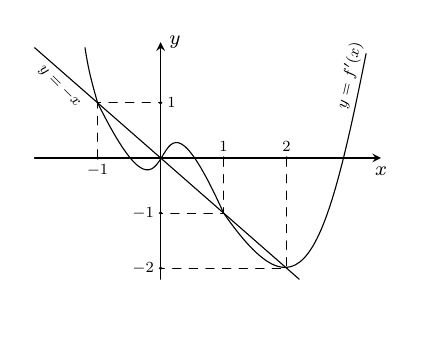
\begin{tikzpicture}[>=stealth,line join=round,line cap=round,font=\footnotesize,smooth,xscale=.8,yscale=0.7]
\draw[->](-2,0)--(3.5,0)node[scale=.9,below]{$x$};
\draw[->](0,-2.2)--(0,2.1)node[scale=.9,right]{$y$};
\draw (-1.2,2) to [out=-82.5,in=104] (-1,1)..controls(0.38237, -2.18977) and (-0.30141, 2.29017)..(1,-1)..controls (2.2073,-2.97669)and (2.59212,-1.96818)..(3.26177,1.89334);
\draw (-2,2)--(2.2,-2.2) (3,1.5)node[rotate=77,scale=0.7]{$y=f'(x)$}
(-1.6,1.3)node[rotate=-45,scale=0.7]{$y=-x$}

;
\fill (0,0)  circle (0.03) 
(-1,0)circle (0.03) node[scale=0.7, below]{$-1$}
(1,0)circle (0.03) node[scale=0.7, above]{$1$}
(2,0)circle (0.03) node[scale=0.7, above]{$2$}
(0,-1)circle (0.03) node[scale=0.7, left]{$-1$}(0,1)circle (0.03) node[scale=0.7, right]{$1$}
(0,-2)circle (0.03) node[scale=0.7,left]{$-2$}
;
\draw[dashed] (-1,0)|-(0,1)  (1,0)|-(0,-1) (2,0)|-(0,-2) ;
\end{tikzpicture}}
\noindent Từ vị trí (trên hoặc dưới) của đồ thị hàm số $y=f'(x)$ so với đường thẳng $y=-x$ trên trục tọa độ, ta có bảng xét dấu của $g'(x)$ như sau
\begin{center}
	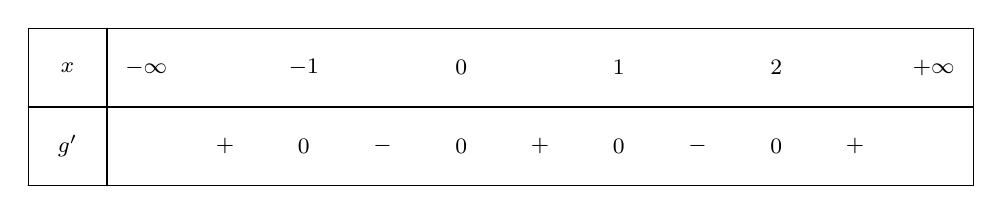
\begin{tikzpicture}[>=stealth,line join=round,line cap=round,font=\footnotesize,scale=1]
	\begin{scope}[shift={(-.5,.5)}]
	\def\a{12}
	\def\b{2}
	\draw (0,0) rectangle+(\a,-\b)
	(0,-1)--+(0:\a)
	(0,-2)--+(0:\a)
	(1,0)--+(-90:\b)	
	;
	\end{scope}
	\path (0,0)node{$x$}+(1,0)node{$-\infty$}+(3,0)node{$-1$}  +(5,0)node{$0$}+(7,0)node{$1$}+(9,0)node{$2$}+(11,0)node{$+\infty$}
	++(0,-1)node{$g'$}
	++(2,0)node{$+$}
	++(1,0)node{$0$}
	++(1,0)node{$-$}
	++(1,0)node{$0$}
	++(1,0)node{$+$}
	++(1,0)node{$0$}
	++(1,0)node{$-$}
	++(1,0)node{$0$}
	++(1,0)node{$+$}
	%	+(5,0)node{$0$}	
	;	
	\end{tikzpicture}
\end{center}
Vậy hàm số $y=g(x)$ nghịch biến trên các khoảng $(-1;0)$, $(1;2)$.
}
\end{ex}

\begin{ex}%[Thi giữa kỳ 1, trường THPT Nguyễn Dục,Sở GD và ĐT - Quảng Nam, năm 2020 - 2021]%[Ninh Tiến Nam, 12EX32021]%[2H1K3-2]
	Cho khối chóp tam giác đều $S.ABC$ có cạnh đáy bằng $a$, góc tạo bởi mặt bên và mặt đáy bằng $60^\circ$. Tính thể tích khối chóp $S.ABC$.
	\choice
	{\True $\dfrac{a^3\sqrt{3}}{24}$}	{$\dfrac{9a^3\sqrt{2}}{4}$}	{$\dfrac{a^3\sqrt{3}}{72}$}	{$\dfrac{2a^3\sqrt{2}}{3}$}
	\loigiai{
		\immini{Gọi $O$ là tâm của tam giác  $ABC$, $M$ là trung điểm của  $AB$.\\
Do $S.ABC$ là khối chóp tam giác đều cạnh đáy bằng $a$ nên ta có $SO\perp (ABC)$.\\	
Xét $\triangle ABC$, ta có $OM=\dfrac{1}{3}CM=\dfrac{1}{3}\cdot\dfrac{a\sqrt{3}}{2}=\dfrac{a\sqrt{3}}{6}$.\\
Dễ thấy, góc tạo bởi mặt bên $(SAB)$ và mặt phẳng đáy $(ABC)$ là góc $\widehat{SMO}$, nên $\widehat{SMO}=60^\circ$.\\
Xét tam giác vuông $SMO$, ta có \[SO=OM\tan \widehat{SMO}=\dfrac{a\sqrt{3}}{6}\cdot \sqrt{3}=\dfrac{a}{2}.\]
}{\begin{tikzpicture}[>=stealth,line join=round,line cap=round,font=\footnotesize,scale=.9]
			\path 
			
			(3,1)coordinate (C)
			(-3,1)coordinate (A)
				(-1,-1)coordinate (B)
				(-.3,4)coordinate (S)
				($(A)!.5!(B)$)coordinate (M)
				($(C)!2/3!(M)$)coordinate (O)
			;
			\draw (A)--(B)--(C)--(S)--cycle (M)--(S)--(B);
			\draw[dashed] (A)--(C) (S)--(O)(M)--(C);
			\foreach \x/\g in {S/90,A/180,B/-90,C/0,O/-90,M/180}\fill (\x)circle (0.03)+(\g:3mm)node[scale=.9]{$\x$};
			\tkzMarkRightAngles(A,M,S S,O,M)
			\end{tikzpicture}}
	\noindent Vậy thể tích khối chóp $S.ABC$ bằng 
	\[V=\dfrac{1}{3}\cdot SO\cdot S_{ABC}=\dfrac{1}{3}\cdot \dfrac{a}{2}\cdot \dfrac{a^2\sqrt{3}}{4}=\dfrac{a^3\sqrt{3}}{24}.\]	
	}
\end{ex}

\begin{ex}%[Thi giữa kỳ 1, trường THPT Nguyễn Dục,Sở GD và ĐT - Quảng Nam, năm 2020 - 2021]%[Ninh Tiến Nam, 12EX32021]%[2H1K3-2]
Tính thể tích của khối chóp tứ giác $S.ABCD$, biết $ABCD$ là hình chữ nhật, $AD=8a$,
$AC=10a$, tam giác $SAB$ đều và nằm trong mặt phẳng vuông góc với đáy.	
	\choice
	{$24a^3\sqrt{3}$}	{$16a^3\sqrt{3}$}	{\True $48a^3\sqrt{3}$}	{$27a^3\sqrt{3}$}	
	\loigiai{
	\immini{
Xét hình chữ nhật $ABCD$, ta có $$AB=\sqrt{AC^2-AD^2}=\sqrt{(10a)^2-(8a)^2}=6a.$$
Gọi $M$ là trung điểm của $AB$.
Do tam giác $SAB$ đều và nằm trong mặt phẳng vuông góc với đáy nên $SM\perp (ABCD)$ và \[SM=\dfrac{\sqrt{3}}{2} AB=\dfrac{\sqrt{3}}{2}\cdot 6a=3a\sqrt{3}.\]}{\begin{tikzpicture}[>=stealth,line join=round,line cap=round,font=\footnotesize,scale=.9]
		\path 
		
		(1,1)coordinate (D)
		(-2.5,1)coordinate (A)
		(-1,-1)coordinate (B)
		($(A)!.5!(B)$)coordinate (M)
		(M)+(90:3)coordinate (S)
		($(B)-(A)+(D)$)coordinate (C)
		;
		\draw (S)--(A)--(B)--(C)--(D)--cycle (S)--(B)(S)--(D)(S)--(C)(S)--(M);
		\draw[dashed] (A)--(D) (A)--(C);
		\foreach \x/\g in {S/90,A/180,B/-90,C/0,M/190,D/20}\fill (\x)circle (0.04)+(\g:3mm)node[scale=.9]{$\x$};
		\tkzMarkRightAngles(A,M,S A,B,C B,C,D C,D,A)
		\end{tikzpicture}}	
\noindent Vậy thể tích khối chóp $S.ABCD$	 bằng
\[V=\dfrac{1}{3}\cdot SM\cdot S_{ABCD}=\dfrac{1}{3}\cdot 3\sqrt{3}a\cdot 6a\cdot 8a=48a^3\sqrt{3}.\]	
	}
\end{ex}

\begin{ex}%[Thi giữa kỳ 1, trường THPT Nguyễn Dục,Sở GD và ĐT - Quảng Nam, năm 2020 - 2021]%[Ninh Tiến Nam, 12EX32021]%[2H1K3-3]
	Cho khối lăng trụ tam giác $ABC.A'BC'$, $M$ là điểm thoả mãn $\overrightarrow{MC'}+2\overrightarrow{MC}=\overrightarrow{0}$. Mặt phẳng
	$(A'BM)$ chia khối lăng trụ thành $2$ phần, gọi $V$ là thể tích phần chứa điểm $A$. Tính $V$ biết thể tích	khối lăng trụ $ABC.A'B'C'$ bằng $18$.
	\choice
	{$5$}{$10$}{\True  $8$}{$12$}	
	\loigiai{
	\immini{
Ta có $V_{B.A'B'C'}=\dfrac{1}{3}S_{A'B'C'}\cdot \mathrm{d}\left(B,(A'B'C') \right) =\dfrac{1}{3}V_{ABC.A'B'C}$,\\suy ra $ V_{B.ACC'A'}=\dfrac{2}{3}V_{ABC.A'B'C}$.\\	
Mặt khác, ta lại có $\overrightarrow{MC'}+2\overrightarrow{MC}=\overrightarrow{0}$ nên $S_{CMA'A}=\dfrac{2}{3}S_{CC'A'A}$.\\ Do đó,
\[V=V_{B.CMA'A}=\dfrac{2}{3}V_{B.ACC'A'}=\dfrac{4}{9}V_{ABC.A'B'C}=\dfrac{4}{9}\cdot 18=8.\]
}{\begin{tikzpicture}[>=stealth,line join=round,line cap=round,font=\footnotesize,scale=1]
\begin{scope}

	\def\h{2}	\path 
		(0,0)coordinate (A)
		+(0:4)coordinate (B)
		+(50:2)coordinate (C)
		(A)--+(-90:\h)coordinate (A')
		(B)--+(-90:\h)coordinate (B')
		(C)--+(-90:\h)coordinate (C')
		($(C)!1/3!(C')$)coordinate (M)
		;	
		\draw (A)--(B)--(C)--cycle (A')--(B') (A)--(A')--(B)--(B');
		\draw[ dashed] (A')--(C')--(B') (C)--(C')(A')--(M)--(B)--(C');
		\foreach \x/\g in {A/180,B/0,C/90,A'/180,B'/0,C'/180,M/30}\fill (\x)circle (0.04)+(\g:3mm)node[scale=.9]{$\x$};\end{scope}
		\end{tikzpicture}}	
			}
\end{ex}

\begin{ex}%[Thi giữa kỳ 1, trường THPT Nguyễn Dục,Sở GD và ĐT - Quảng Nam, năm 2020 - 2021]%[Ninh Tiến Nam, 12EX32021]%[2D1G2-4]
Có hai giá trị của tham số $m$ là $m_1,$ $m_2$ để đường thẳng qua hai điểm cực trị của đồ thị hàm số $y=x^3-3mx+2$ cắt đường tròn tâm $I(1;1)$ bán kính $R=1$ tại hai điểm phân biệt $A$, $B$ sao cho diện tích
tam giác $IAB$ đạt giá trị lớn nhất. Tổng $m_1+ m_2$ bằng	
	\choice
	{$\dfrac{2}{3}$}{\True $2$}{ $\dfrac{4}{3}$}{$1$}	
	\loigiai{
		Ta có $y'=3x^2-3m$ và $y=\dfrac{1}{3}x\cdot y'-2mx+2$.\\
		 Hàm số có hai cực trị khi và chỉ khi $m>0$, khi đó phương trình đường thẳng đi qua hai điểm cực trị là $d\colon y=-2mx+2$, ($m>0$).
\immini{Gọi $H$ là hình chiếu vuông góc của $I$ lên $d$.\\
Ta có
		 \[AH=\mathrm{d}\left(I,d \right)=\dfrac{|2m\cdot 1+1-2|}{\sqrt{4m^2+1}}= \dfrac{|2m-1|}{\sqrt{4m^2+1}}.\]
		 Đường thẳng $d$ cắt đường tròn $(I;R)$ tại hai điểm phân biệt khi và chỉ khi $IH<1$.\hfill$(*)$\\
Với điều kiện $(*)$, ta có đánh giá về diện tích tam giác $IAB$ như sau
}{\begin{tikzpicture}[>=stealth,line join=round,line cap=round,font=\footnotesize,scale=1]
	\begin{scope}[scale=.8]
	
	 \path (1,1)coordinate(I)
		 +(40:2)coordinate(A)
		 +(150:2)coordinate(B)
		 ($(A)!(I)!(B)$)coordinate(H)
		 ($(A)!1.4!(B)$)coordinate(C)
		  ($(B)!1.4!(A)$)coordinate(D)
		 ;
		 \draw (A)--(I)--(B)--cycle (D)--(C) (I)circle(2) (I)--(H);
		 \foreach \x/\g in{A/40,B/100,I/-90,H/90}\fill (\x) circle(0.03)+(\g:3mm)node[scale=.9]{$\x$};\tkzMarkRightAngle(I,H,B)
		 \end{scope}	
		 \end{tikzpicture}}
\noindent \[S_{IAB}=\dfrac{1}{2}IA\cdot IB\cdot\sin \widehat{AIB}\le \dfrac{1}{2}\cdot 1\cdot 1\cdot 1=\dfrac{1}{2}.\]		
Dấu \lq\lq$=$\rq\rq\ xảy ra khi và chỉ khi $\sin \widehat{AIB}=1\Leftrightarrow\widehat{AIB}=90^\circ$.\\
Điều này tương đương với
\allowdisplaybreaks
\begin{eqnarray*}
	IH=\dfrac{IB}{\sqrt{2}}\Leftrightarrow \dfrac{|2m-1|}{\sqrt{4m^2+1}}=\dfrac{1}{\sqrt{2}}\Leftrightarrow 4m^2-8m+1=0\Leftrightarrow m=1\pm\dfrac{\sqrt{3}}{2}.
\end{eqnarray*}
Hiển nhiên  $m=1+\dfrac{\sqrt{3}}{2}$, $m=1-\dfrac{\sqrt{3}}{2}$  thỏa mãn $(*)$  và điều điện $m>0$. \\Vậy $m_1+m_2=2$.	}
\end{ex}


\Closesolutionfile{ans}
\begin{indapan}{10}
	{ans/ans-2-GHK1-29-NguyenDuc-QuangNam-21}
\end{indapan}